
\documentclass[11pt,a4paper]{report}                                   

\usepackage[T1]{fontenc}
\usepackage{kpfonts}
\usepackage[utf8]{inputenc}
\usepackage[hyphens]{url}
\usepackage{graphicx}
\usepackage{a4}
\usepackage[english]{babel}
\usepackage{subfiles}
\usepackage{acronym}
\usepackage{tocbibind}
\usepackage{cmap}
\usepackage{listingsutf8}
\usepackage{color}

\newcommand{\thema}{Architektur für ein webbasiertes graphisches Modellierungsframework}
\newcommand{\schlagworte}{Modelgetriebene Softwareentwicklung, Webapplikation, Architektur}
\newcommand{\zusammenfassung}{TBD}
\newcommand{\ausgabedatum}{01.10.2017}
\newcommand{\abgabedatum}{01.04.2018}
\newcommand{\autor}{Philipp Daniels}
\newcommand{\autorStrasse}{Rheingutstraße 30}
\newcommand{\autorPLZ}{78462}
\newcommand{\autorOrt}{Konstanz}
\newcommand{\autorGeburtsort}{Mannheim}
\newcommand{\autorGeburtsdatum}{03.02.1989}
\newcommand{\prueferA}{Prof. Dr. Marko Boger}
\newcommand{\prueferB}{Prof. Dr. Markus Eiglsperger}
\newcommand{\firma}{HTWG}
\newcommand{\studiengang}{Master of Science Informatik}

%PDF linking package
\usepackage[hidelinks,breaklinks=true]{hyperref}
% hyperref customization
\hypersetup{
    pdftitle    ={\thema}, % title
    pdfsubject	={\thema}, % subject of the document
    pdfauthor	={\autor}, % author
    pdfkeywords	={}, % list of keywords
    pdfcreator	={}, % creator of the document
    pdfproducer	={}, % producer of the document
    colorlinks=false, % false: boxed links; true: colored links
    linkcolor=red, % color of internal links (change box color with linkbordercolor)
    citecolor=green, % color of links to bibliography
    filecolor=magenta, % color of file links
    urlcolor=cyan, % color of external links
    unicode=true, % non-Latin characters in Acrobat’s bookmarks
    pdftoolbar=true, % show Acrobat’s toolbar?
    pdfmenubar=true, % show Acrobat’s menu?
    pdffitwindow=false, % window fit to page when opened
    pdfnewwindow=true % links in new PDF window
}

\definecolor{lightgray}{rgb}{.9,.9,.9}
\definecolor{darkgray}{rgb}{.4,.4,.4}
\definecolor{purple}{rgb}{0.65, 0.12, 0.82}
\lstdefinelanguage{JavaScript}{
  keywords={break, case, catch, class, continue, const, constructor, debugger, default, delete, do, else, export, false, finally, for, function, get, if, import, in, instanceof, let, new, null, return, switch, this, throw, true, try, typeof, var, void, while},
  morecomment=[l]{//},
  morecomment=[s]{/*}{*/},
  morestring=[b]',
  morestring=[b]",
  keywordstyle=\color{blue}\bfseries,
  identifierstyle=\color{black},
  commentstyle=\color{purple}\ttfamily,
  stringstyle=\color{red}\ttfamily,
  sensitive=true
}

\lstset{
    basicstyle=\footnotesize,
    breakatwhitespace=false,
    breaklines=true,
    captionpos=b,
    frame=single,
    keepspaces=true,
    numbers=left,
    numbersep=5pt,
    showspaces=false,
    showstringspaces=false,
    showtabs=false,
    stepnumber=1,
    tabsize=2,
    title=\lstname,
    inputencoding=utf8/latin1
}

\newcommand{\theHchoice}{\arabic{question}.\arabic{choice}}

\begin{document}

\hypersetup{pageanchor=false}


\begin{titlepage}

\vspace*{-3.5cm}

\begin{flushleft}
\hspace*{-1cm} 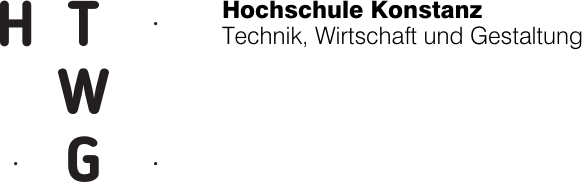
\includegraphics[width=10cm]{htwg-logo.png}
\end{flushleft}

\vspace{2.5cm}

\begin{center}
	\huge{
		\textbf{\thema} \\[5cm]
	}
	\Large{
		\textbf{\autor}} \\[6.5cm]
	\large{
		\textbf{Konstanz, \abgabedatum} \\[2.3cm]
	}
	
	\Huge{
		\textbf{{\sf MASTERARBEIT}}
	}
\end{center}

\end{titlepage}

\thispagestyle{empty}
{
\setlength{\parskip}{0.5cm}
        \begin{center}
        \textbf{\huge MASTERARBEIT}

        \textbf{zur Erlangung des akademischen Grades}

        \textbf{\Large Master of Science (M. Sc.)}

        \textbf{an der}

        \textsf{\huge Hochschule Konstanz}\\
        {\small Technik, Wirtschaft und Gestaltung}

        \textsf{\Large Fakultät Informatik} \\
        Studiengang \studiengang
        \end{center}
}
\begin{center}

\vspace*{2cm}

\begin{tabular}{p{3cm}p{10cm}}
Thema: & \textbf{\large \thema} \\[15ex]
Masterkandidat: & \autor, \autorStrasse, \autorPLZ\ \autorOrt \\[15ex]
1. Prüfer: & \prueferA \\
2. Prüfer: & \prueferB \\[25ex]
Ausgabedatum: & \ausgabedatum \\
Abgabedatum: & \abgabedatum \\
\end{tabular}
\end{center}


\hypersetup{pageanchor=true}
\pagenumbering{Roman} 
\setcounter{page}{1}


\chapter*{
  \begin{center}
  {\Large{Zusammenfassung (Abstract)}}
  \addcontentsline{toc}{chapter}{Abstract}
  \end{center}
}

\bigskip

\begin{center}
	\begin{tabular}{p{2.8cm}p{10cm}}
		Thema: & \thema \\
		 & \\
		Masterkandidat: & \autor \\
		 & \\
		Firma: & \firma \\
		 & \\
		Betreuer: & \prueferA  \\[.5ex]
		 &  \prueferB \\
		 & \\
		Abgabedatum: & \abgabedatum \\
		 & \\
		Schlagworte: & \schlagworte \\
		 & \\
	\end{tabular}
\end{center}

\bigskip

\noindent
\zusammenfassung

%
% TABLE OF CONTENTS
%
\renewcommand{\contentsname}{Inhaltsverzeichnis}
\tableofcontents
\thispagestyle{plain}
\newpage

\chapter*{Abkürzungsverzeichnis}
\label{chap:ACRONYM}
\addcontentsline{toc}{chapter}{Abkürzungsverzeichnis}

\begin{acronym}[Bash]
  \acro{lxc}[LXC]{Linux Container}
  \acro{vm}[VM]{Virtual Machine}

\end{acronym}

\newpage

\label{chap:FIGURES}
\renewcommand\listfigurename{Abbildungsverzeichnis}
\listoffigures
\newpage


\label{chap:LIST_OF_LISTINGS}
\renewcommand\lstlistlistingname{Quelltextverzeichnis}
\lstlistoflistings
\newpage



%Content
\pagenumbering{arabic} 
\setcounter{page}{1}
\setlength{\parindent}{0em}
\setlength{\parskip}{1em}
\renewcommand{\baselinestretch}{1.5}
\renewcommand\chaptername{Kapitel}
\renewcommand{\figurename}{Abbildung}
\chapter{Einleitung}
\label{sec:INTRO}

\section{Problemstellung}
\label{sec:INTRO_PROBLEM}

\section{Wissenschaftliche Fragestellung}
\label{sec:INTRO_SCIENTIFIC_QUESTION}

\section{Aufbau}
\label{sec:INTRO_STRUCTURE}


\chapter{Grundlagen}
\label{sec:FUNDAMENTALS}

In diesem Kapitel werden die Grundlagen für diese Arbeit vorgestellt. Zu diesen Grundlagen gehört zuerst einmal die Einordnung des Begriffs Softwarearchitektur. Des Weiteren wird noch auf die Technologie der Containervirtualisierung eingegangen.

\section{Softwarearchitektur}
\label{sec:FUNDAMENTALS_ARCHITECTURE}

Der Vorgang zur Erstellung der Architektur einer Software, auch Softwarearchitektur genannt, wird definiert als Prozess des Entwerfens, Definierens, Ausdrucks, Dokumentierens, Kommunizierens, Zertifizierens der korrekten Implementierung, Wartung und Verbesserung einer Architektur während des gesamten Lebenszyklus eines Systems \cite{ISO_IEC_42010}. Dabei besteht die Softwarearchitektur aus den grundlegenden Konzepten oder Eigenschaften eines Systems in seiner Umgebung, verkörpert in seinen Elementen, Beziehungen und in den Prinzipien seines Designs und seiner Entwicklung. Weiterhin ist die Umgebung eines Systems ein Kontext, der die Einstellung und die Umstände aller Einflüsse auf ein System bestimmt. Die Umgebung eines Systems umfasst entwicklungspolitische, technologische, betriebswirtschaftliche, betriebliche, organisatorische, politische, ökonomische, rechtliche, regulatorische, ökologische und soziale Einflüsse.

Die Softwarearchitektur gehört zum Themenfeld des Softwareentwurfs. Jedoch ist nicht alles in einem Softwareentwurf auch gleichzeitig ein Teil der Softwarearchitektur. Vereinfacht dargestellt, bietet die Softwarearchitektur eine strukturelle Übersicht einer Software und beinhaltet Lösungen für strukturelle Entscheidungen, die sich im nachhinein nur mit sehr viel Aufwand ändern lassen. Die Softwarearchitektur ist somit ein grober Entwurf und lässt sich von einem Detailentwurf einer Software abgrenzen. Formal lässt sich eine genaue Trennung der Entwürfe jedoch nur schwer definieren.

\section{Modellgetriebene Softwareentwicklung}
\label{sec:FUNDAMENTALS_MDSD}

Die Anwendung von Modellen in der Softwareentwicklung hat eine lange Tradition und ist seit der Entwicklung der \ac{uml} noch populärer geworden, die Beziehung zwischen Modell und Softwareimplementierung ist nur bewusst, aber nicht formal \cite[S. 3-4]{mdsd}. Sie hat zwei gravierende Nachteile: Zum einen sind Softwaresysteme nicht statisch und unterliegen insbesondere in den ersten Phasen ihres Lebenszyklus erheblichen Veränderungen. Die Dokumentation muss daher akribisch angepasst werden, was eine komplexe Aufgabe sein kann - je nachdem, wie detailliert sie ist - oder sie wird inkonsistent. Andererseits fördern solche Modelle nur indirekt den Fortschritt, da es die Interpretation des Software-Entwicklers ist, die schließlich zu implementierten Programmcode führt. Das sind die Gründe, warum - verständlicherweise - viele Programmierer Modelle als Overhead und bestenfalls als Zwischenergebnisse betrachten. \ac{mdsd} hat einen ganz anderen Ansatz: Modelle stellen keine Dokumentation dar, sondern sind dem Code gleichgestellt, da ihre Implementierung automatisiert ist. \ac{mdsd} zielt daher darauf ab, domänenspezifische Abstraktionen zu finden und durch formale Modellierung zugänglich zu machen. Dieses Verfahren schafft ein großes Potenzial für die Automatisierung der Softwareproduktion, was wiederum zu einer Steigerung der Produktivität führt. Darüber hinaus steigt sowohl die Qualität als auch die Wartbarkeit von Softwaresystemen. Modelle können auch von Fachleuten verstanden werden. Um das domänenspezifische Modellkonzept erfolgreich anwenden zu können, müssen drei Voraussetzungen erfüllt sein: Domänenspezifische Sprachen sind erforderlich, um die eigentliche Formulierung von Modellen zu ermöglichen, Sprachen, die die notwendigen \ac{m2t} Transformationen ausdrücken können, und Compiler, Generatoren oder Transformatoren, die die Transformationen ausführen können, um auf verfügbaren Plattformen ausführbaren Code zu erzeugen.

Eine \ac{dsl} dient dazu, die wesentlichen Aspekte einer Domain - aber nicht alle denkbaren Inhalte - formal ausformulierbar und modellierbar zu machen \cite[S. 58]{mdsd}. Dazu besitzt es ein Metamodell einschließlich seiner statischen Semantik und eine entsprechende konkrete Syntax. Das allein reicht nicht aus: Die dynamische Semantik, die notwendig ist, um den Konstrukten des Metamodells einen Sinn zu geben, fehlt noch. Die Semantik eines \ac{dsl} ist in mehrfacher Hinsicht relevant: Einerseits muss der Modellierer die Bedeutung der ihm zur Verfügung stehenden Sprachelemente kennen, um sinnvolle Modelle erstellen zu können, andererseits müssen automatische Transformationen der Modelle genau diese Semantik ausführen. \acp{dsl} können in ihrer Leistung und Komplexität variieren. Einfache textuelle Konfigurationsmöglichkeiten mit Gültigkeitstests können eine \ac{dsl} bilden, während am anderen Ende des Spektrums grafische Sprachen mit entsprechenden sprachspezifischen Editoren sein können.

\section{Webapplikation}
\label{sec:FUNDAMENTALS_WEB}

Webapplikationen laufen nicht wie eine klassische Desktopanwendung lokal auf dem eigenen PC, sondern wird auf einem Server ausgeführt und können über das Internet in einem Web Browser zugegriffen werden \cite{web_application}. Die Datenverarbeitung und -persistierung findet auf dem Server statt und die Darstellung findet wiederum im Webbrowser als Client statt. Dabei werden Daten und der Programmcode über \ac{http} übertragen. Eine Webapplikation entspricht somit einer Client-Server Architektur.

In \ac{ria} reagiert die Webseite dynamisch auf Benutzereingaben \cite{rich_internet_application}. Dies wird entweder durch proprietäre Lösung auf Basis von z.B. \textit{Flash} oder \textit{Microsoft Silverlight} oder durch den starken Einsatz von JavaScript wie z.B. mit der Bibliotheken \textit{jQuery} ermöglicht. Inzwischen kommen die proprietären Lösungen immer seltener zum Einsatz und werden nach und nach eingestellt, da \ac{html} immer mehr dieselben Funktionen von sich aus anbietet \cite{flash_end_of_life}.

\ac{spa} ist einer spezielle Art von Webapplikationen, die noch stärker einer Desktopanwendung ähnelt, da nicht mehr wie sonst eine Webseite aus untereinander referenzierten Dokumenten besteht, sondern nur noch aus einem einzigen Dokument \cite[S.~497]{javascript_definitive_guide}. Bei einer Benutzerinteraktion werden die Inhalte entsprechend dynamisch im Hintergrund nachgeladen. Dieser Ansatz ermöglicht die Entwicklung von Fat-Clients durch eine immer stärker werdende Verschiebung von Logik aus dem Server zum Client. Dies führt entsprechend zu Entlastung des Servers und gleichzeitig größeren Belastung des Web Browsers auf Seiten des Clients.

\section{Containervirtualisierung}
\label{sec:FUNDAMENTALS_CONTAINER}

In der Informatik bezeichnet der Begriff Virtualisierung ein Framework zur Trennung der Ressourcen eines Computers in mehrere Ausführungsumgebungen \cite{virtualization}. Dies kann durch Konzepte oder Technologien wie Hard- oder Software-Partitionierung, Time-Sharing, teilweise oder gänzliche Maschinensimulation oder auch -emulation realisiert werden. Dabei existieren verschiedene Arten der Virtualisierung. Bei der Hardwarevirtualisierung oder Emulation geht es um den Computers als gesamte Hardware Plattform \cite{wiki:hardware_virtual}. Dadurch ist es möglich parallel neben einem fest installiertem Betriebssystem, auch Hostsystem genannt, auf einem Computer weitere simulierte Computerumgebungen mit einem Betriebssystem als Gastsystem auszuführen. Diese werden allgemein auch als \ac{vm} bezeichnet. Dabei besteht keine Einschränkung hinsichtlich des genutzten Betriebssystems als Gastsystem. Somit ist es möglich z.B. auf einem Hostsystem mit Windows ein Gastsystem mit einem Linux basiertem Betriebssystem zu betreiben. Der umgekehrte Fall ist entsprechend auch möglich. Des Weiteren sind aufgrund der Abstraktionsschicht durch die Virtualisierung die einzelnen \acp{vm} vom Hostsystem und anderen Gastsystemen isoliert und ein Zugriff auf diese wird unterbunden. Die vollständige Isolierung konnte jedoch selbst in der jüngsten Vergangenheit nicht immer zu 100\% sichergestellt werden \cite{CVE-2017-4934}.

Eine weitere Art der Virtualisierung wird als Software- oder auch Containervirtualisierung bezeichnet \cite{software_container}. Historisch hat sich die Containervirtualisierung aus der Unix-System Operation \textit{chroot} entwickelt. Die \textit{chroot} ermöglicht die Zugriffe eines Prozesses auf ein Unterverzeichnis zu limitieren. Aus den Konzepten der \textit{chroot} Operation haben sich die heutigen \ac{lxc} entwickelt. \ac{lxc} bauen auf Standardfunktionalitäten des Linux Kernels auf und isolieren anhand von Kernel Namespaces und \textit{cgroups} die Ausführung eines Programms. Kernel Namespaces isolieren dabei mit eigenen Prozess-IDs, Dateisystem, Netzwerk und Benutzer-IDs ein Programm vom Hostsystem. Wiederum limitieren und priorisieren \textit{cgroups} die Ressourcen eines Computers wie z.B. CPU, Arbeitsspeicher oder Netzwerk. Anders als bei einer \ac{vm} wird nicht ein ganzes Betriebssystem in einer virtualisierten Umgebung ausgeführt, sondern, wie in Abbildung~\ref{fig:DOCKER_VS_VM} auf Seite~\pageref{fig:DOCKER_VS_VM} zusehen, nur einzelne Programme. Dabei kann ein Programm aus einem Hauptprozess und mehreren Subprozessen bestehen. Die virtuelle Umgebung eines einzelnen Programms wird als Container bezeichnet. Container haben in vielen Szenarien signifikante Geschwindigkeitsvorteile gegenüber \acp{vm} \cite{performance_container}. Neben den Ressourcen eines Computers nutzen alle Container denselben Betriebssystem Kernel. Jedoch können verschiedene Linux Distributionen unabhängig vom Hostsystem innerhalb der Container zur Verfügung gestellt werden. Somit findet die Virtualisierung der Container auf der Ebene des Betriebssystems statt und ist im Fall von \ac{lxc} von bestimmten Funktionalitäten des Linux Kernels abhängig. Dank \ac{lxc} ist die Containervirtualisierung auf allen Linux basierten Distributionen möglich, aber es ist auch genau auf diese limitiert und die Portabilität auf andere Kernel bedingt die Unterstützung einer ähnlichen Funktionalität zur Virtualisierung auf Ebene des Betriebssystems.

\begin{figure}
    \centering
    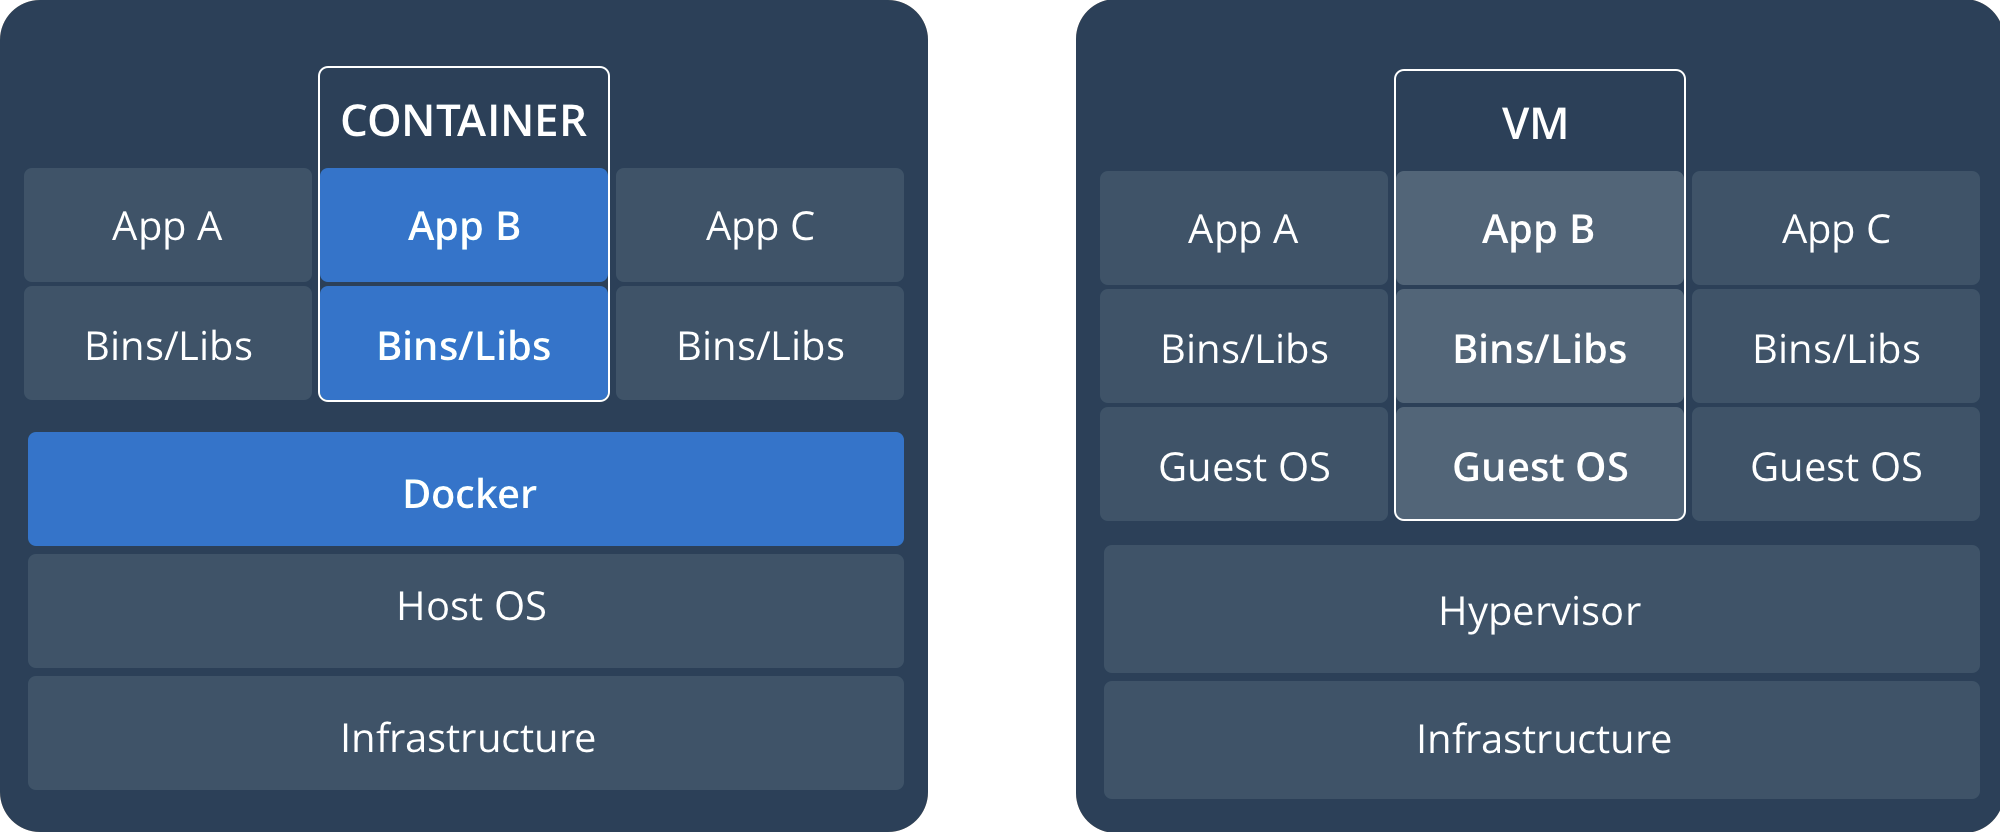
\includegraphics[width=4in]{figures/docker-vs-vm.png}
    \caption[Docker VS VM]
    {Docker VS VM \cite{what_container}}
    \label{fig:DOCKER_VS_VM}
\end{figure}

Die Open Source Plattform \textit{Docker} ist neben vielen anderen Lösungen einer der bekanntesten Vertreter der Containervirtualisierung und ist Gründer der \textit{Open Container Initiative} \cite{about_docker}. Erstmals wurde \textit{Docker} von seinem Erfinder Solomon Hykes im Jahr 2013 der Öffentlichkeit vorgestellt und hat inzwischen die Art und Weise, wie Anwendungen besonders bei Firmen mit vielen Hosts betrieben werden, revolutioniert \cite{docker_adoption}. Durch einen modularen Aufbau und einer Kooperation mit Microsoft unterstützt \textit{Docker} neben einer Variante mit einer Linux \ac{vm} inzwischen eine native Containervirtualisierung auf Windows \cite{docker_for_windows}. Über den kostenlosen \textit{Docker Compose} Client lassen sich mehrere unterschiedliche Container zu einem Bundle zusammenfassen \cite{docker_compose} und ermöglichen somit komplexe Anwendungen mit verschiedenen Diensten, die jeweils ihren eigenen Ausführungsumgebungen haben. Die verschiedenen Dienste können dabei über das Netzwerk isoliert vom Hostsystem miteinander kommunizieren. Dabei muss diese Kommunikation zwischen den Containern so wie die externe Kommunikation jeweils einzeln freigegeben werden und verfolgt somit das Prinzip Secure-by-Default. \textit{Docker} ist jedoch nicht bei einer reinen Containervirtualisierung geblieben. Mit der in den \textit{Docker} Client integrierten Erweiterung \textit{Docker Swarm} können mehrere \textit{Docker} Hosts zu einem einzigen virtuellen Host vereint werden und stellt somit ein Cluster an \textit{Docker} Hosts zur Verfügung \cite{docker_swarm}. Dabei wird per Default die Kommunikation zwischen den \textit{Docker} Hosts mit TLS verschlüsselt. Für einen \textit{Docker} Client ist es dabei unerheblich, ob nun \textit{Docker} auf demselben Host oder in einem Cluster läuft. Die API bleibt in beiden Szenarien dieselbe und führt zu einem leichten Einstieg mit \textit{Docker Swarm}.

\section{Alternative Ansätze}

Der Bereich der graphischen Modellierung ist bei weitem kein neues Themengebiet und hat schon eine über mehrere Jahrzehnte lange Geschichte \cite{paper_metaedit}. Die \textit{Eclipse Foundation} bietet z.B. mit dem \ac{gmf} die Infrastruktur zur Entwicklung von graphischen Editoren auf Basis des \textit{Eclipse Modeling Frameworks} und des \textit{Graphical Editing Frameworks} \cite{eclipse_gmf}. Das \ac{gmf} dient als Grundlage für eine ganze Reihe von Lösungen im Rahmen der graphischen Modellierung wie z.B. \textit{Sirius} oder auch \textit{Graphiti} \cite{sirius,graphiti}. Eine von \textit{Eclipse Foundation} unabhängige Lösung bietet z.B. das Produkt \textit{MetaEdit+} \cite{metaedit}. Dabei unterstützt \textit{MetaEdit+} zum einen die Erstellung einer eigenen graphischen \ac{dsl} mit entsprechenden Generatoren und zum anderen einen Editor mit dem ein Benutzer auf Basis der eigenen \ac{dsl} Modelle erstellen kann. 

Alle diese Lösungen haben eine Gemeinsamkeit. Egal, ob basierend auf dem \ac{gmf} oder nicht, alle laufen als Anwendung innerhalb eines Desktops. Webbasierte Lösungen im Bereich der graphischen Modellierungsframeworks sind bis zum jetzigen Zeitpunkt noch keine veröffentlich worden. Im Bereich der webbasierten graphischen Editoren mit einer festen \ac{dsl} existieren aber Projekte wie z.B. \textit{Node-RED} von IBM zur Flow-basierten Programmierung für Geräten des Internet of Things \cite{node_red}.

Ein weiteres Thema bei webbasierten graphischen Modellierungsframeworks ist die Ausführung von Benutzer erstellten Programmen auf einem Server im Rahmen der Generatoren. Speziell für Modellierungsframeworks wurde in diesem Bereich noch nichts veröffentlicht. Außerhalb von Modellierungsframework existieren jedoch Projekte die eine große Menge von Benutzer erstellten Programmen regelmäßig ausführen und diese in einer Art und Weise isoliert haben. Ohne dabei Ihre Infrastruktur zu gefährden. Eines dieser Projekte ist z.B. \textit{Travis CI} eine Cloud basierte Lösung für automatisierte Builds von Open Source Projekten \cite{tracis_ci}.


\chapter{Lösung}
\label{sec:SOLUTION}

\section{Modellierungsframework}
\label{sec:SOLUTION_MODEL}

\section{Webapplikation}
\label{sec:SOLUTION_WEB}

\section{Zeta}
\label{sec:SOLUTION_ZETA}


\chapter{Resümee}
\label{sec:SUMMARY}

\section{Schlussfolgerungen}
\label{sec:SUMMARY_CONCLUSION}

\section{Ausblick}
\label{sec:SUMMARY_OUTLOOK}



\renewcommand\thesection{A.\arabic{section}}
\renewcommand\thesubsection{\thesection.\arabic{subsection}}

\chapter*{Anhänge}
\label{chap:APPENDIX}
\addcontentsline{toc}{chapter}{Anhänge}

\pagenumbering{arabic}
\setcounter{page}{1}
\renewcommand{\thepage}{A-\arabic{page}}


\section{Abbildungen}
\label{sec:APPENDIX_FIGURES}

\section{Quelltexte}
\label{sec:APPENDIX_LISTINGS}

\renewcommand{\baselinestretch}{1}

\clearpage


\phantomsection
\renewcommand{\bibname}{Quellenverzeichnis}
\bibliography{references}
\bibliographystyle{apalike}
\newpage


\end{document}
